\documentclass[../main.tex]{subfiles}
\graphicspath{{\subfix{../images/}}}

\begin{document}

\begin{newrequirements}
    \begin{todolist}
    \item[\done] Actual Design description with pictures 
        and diagrams. E.g., a “wiring diagram” 
        of the implemented hardware can be 
        added. 

    \item[\done] Actual images of various modules must 
        be included wherever possible. 
        Otherwise, at least the images of 
        various aspects of the completed design 
        must be shown. 

    \item[\done] List the different tools and framework 
        used for the implementation. 

    \item[\done] Discuss any novel aspects of your 
        implementation (if applicable). You may 
        link this aspect of your design to the 
        comparison table at the end of 
        literature review and elaborate on the 
        steps taken in achieving these 
        novelties in your design. 

    \item [\done] Discuss the challenges encountered 
        during the implementation and how they 
        were addressed. 

    \item [\done] You may organize any of the above 
        recommended points as subsections 

    \end{todolist}
\end{newrequirements}

\subsection{Hardware}

\lipsum[1]

\subsection{Reinforcement learning}

\lipsum[1]

\subsection{User interface}

\begin{figure}[tbp] 
	\centering
	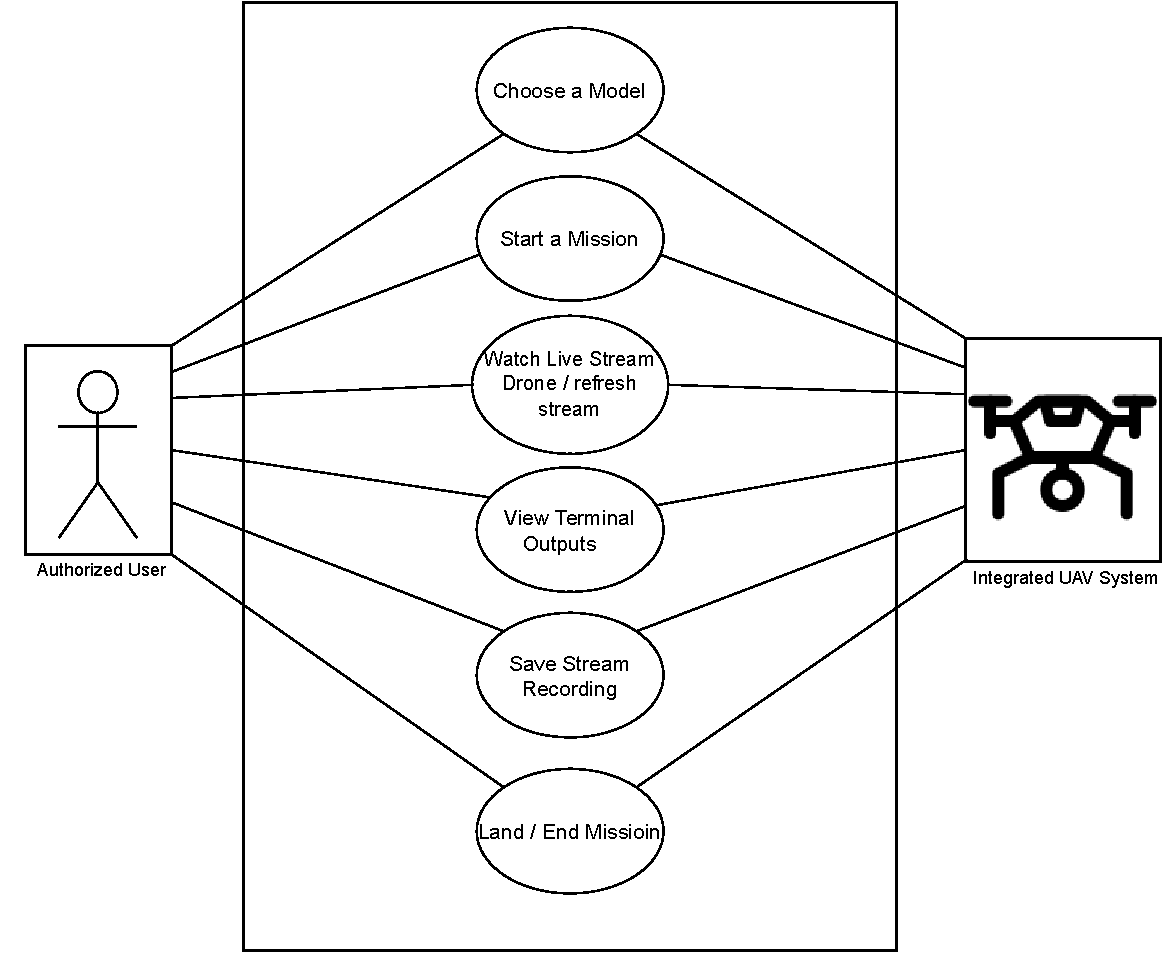
\includegraphics[width=0.9\textwidth]{gui-use-cases} 
	\caption{This use case diagram depicts the different use cases that any authorized users can have using the website.}
	\label{fig:gui-use-cases} 
\end{figure}

Below are the list of use cases that a user can do using the AirEye website as seen in \cref{fig:gui-use-cases} : 
\begin{itemize}	
	\item The user is able to choose a certain model that is available, choosing this model will run a specific script in the drone. 
	\item The user can start the mission.
	\item The user can watch the live stream from the drone camera and refresh the stream in case of any error.
	\item The user can see the outputs of the terminal to keep track of different variables.
	\item The user can save the stream recording. 
	\item The user can end the mission.
\end{itemize}

\begin{figure}[tbp]
	\centering
	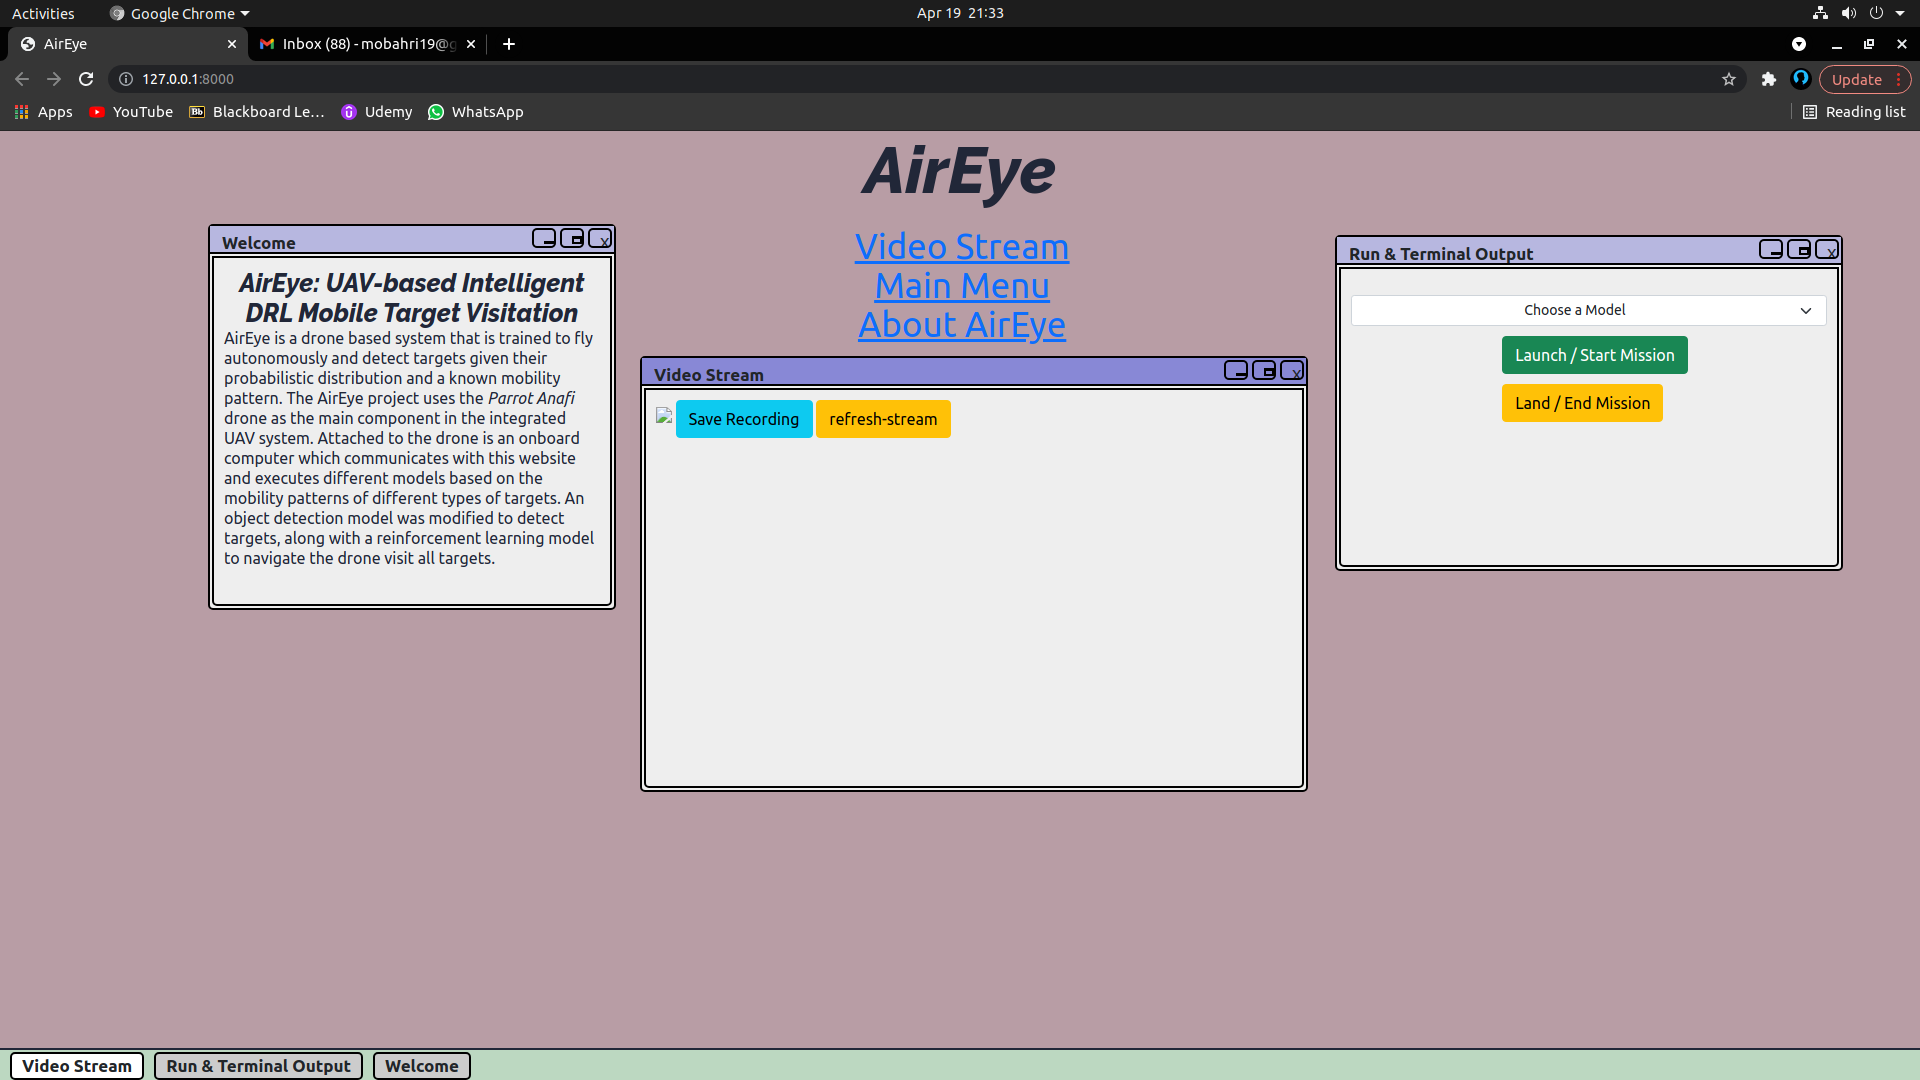
\includegraphics[width=0.99\textwidth]{gui-main-page}
	\caption{The main page of the AirEye website.}
	\label{fig:gui-main-page}
\end{figure}

Many software components were put together to produce what we have in \cref{fig:gui-main-page}, mainly: 
\begin{itemize}
	\item Olympe, the drone controller. 
	\item pyzbar, for \textsc{qr} code detection.
	\item OpenCV, huge computer vision library.
	\item \textsc{html}, \textsc{css}, and javascript for frontend web 
	development.
	\item Python Flask, backend framework.
	\item Gunicorn, \textsc{wsgi} \textsc{http} server
	\item Nginx, reverse proxy and web server. 
\end{itemize}

Many novel aspects were implemented in this website, different models could be 
made and each model is responsible for a certain type of targets, One model 
might be good for mobile targets and another could be better for fixed ones. 
Challenges were mainly faced in the backend as establishing the communication 
between the web server and the frontend was not easy to manage. Also, 
streaming live from the drone's camera to the user interface was 
difficult and new to us.



\end{document}
